\pagebreak 

% ----------------------------------------------------------------
\appendix
\setcounter{figure}{0} \renewcommand{\thefigure}{A.\arabic{figure}}
\setcounter{table}{0} \renewcommand{\thetable}{A.\arabic{table}}
\section{Additional Empirical Results}
\label{sec:appendix}
% ----------------------------------------------------------------


\subsection{Additional results with real-time forecasting of job risks}
\label{appendix:real_time_results_more}


Figure \ref{fig:real_time_ar} compares the real-time machine-efficient forecasts of job risks based on the Lasso with one from an AR(1) model using only the 3-month lag of the realized job flow rate. The two closely move with each other. The mean square errors (MSE) from the two are almost equal for both job finding and separation. This indicates that near-term job risks are highly predictable, especially in normal times. The major exceptions were during the Covid era. 

 \begin{figure}[ht]
    	\caption{Real-time Machine-efficient Risks from Lasso and AR(1)}
    	\label{fig:real_time_ar}
    	\begin{center}
	\adjustimage{max size={0.48\linewidth}}{Figures/predicted_comparison_JF_real_time_ar1.pdf} 
 	\adjustimage{max size={0.48\linewidth}}{Figures/predicted_comparison_JS_real_time_ar1.pdf} 
    	\end{center}
    	
    	\begin{flushleft}\footnotesize{Note: Multi-variate Lasso real-time forecasts versus one from AR(1) model.}\end{flushleft}
    \end{figure}


\subsection{Additional results with imputation of perceived job risks}



\subsubsection{Cross-validation of the imputing methodology}

We evaluate the performance of imputing methods used to backcast SCE job beliefs by examining if the imputed beliefs based on the 2013-2022 in-sample can successfully generate belief backcasts that match the observed expectations in MSC. In particular, Figure \ref{fig:impute_cv_with_msc_separation_inflation} plots the imputed beliefs for two series of expectations on median inflation expectations and 5-year-ahead job separation expectations in MSC based on 2013-2022 in-sample. They have an impressively large degree of comovement with the observed data. We are particularly careful to exclude any indices in MSC that are directly correlated to the target expectation series. They provide a strong external validation of our belief imputation methods. 

 \begin{figure}[ht]
    	\caption{Imputed Beliefs versus Observed Expectations in MSC}
    	\label{fig:impute_cv_with_msc_separation_inflation}
    	\begin{center}
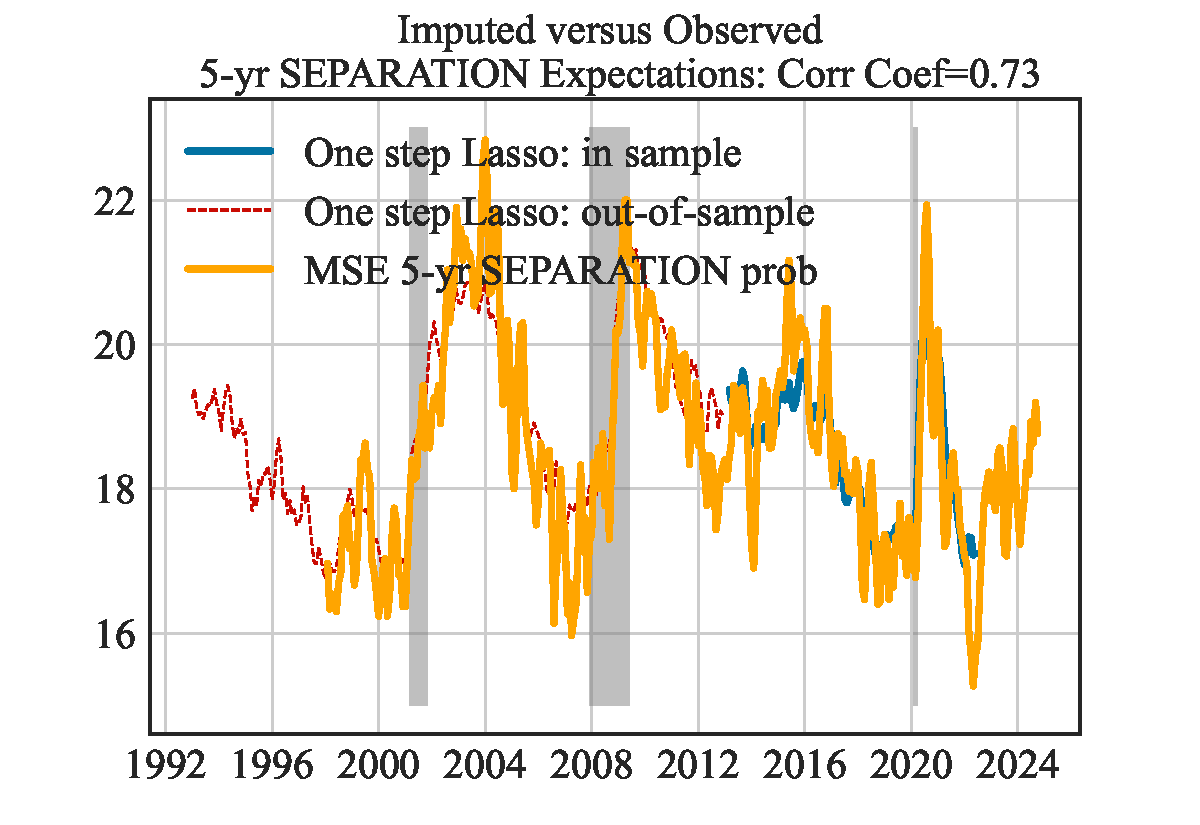
\includegraphics[width=0.49\linewidth]{Figures/imputed_comparison_separation_5y_prob_msc_1step.pdf}  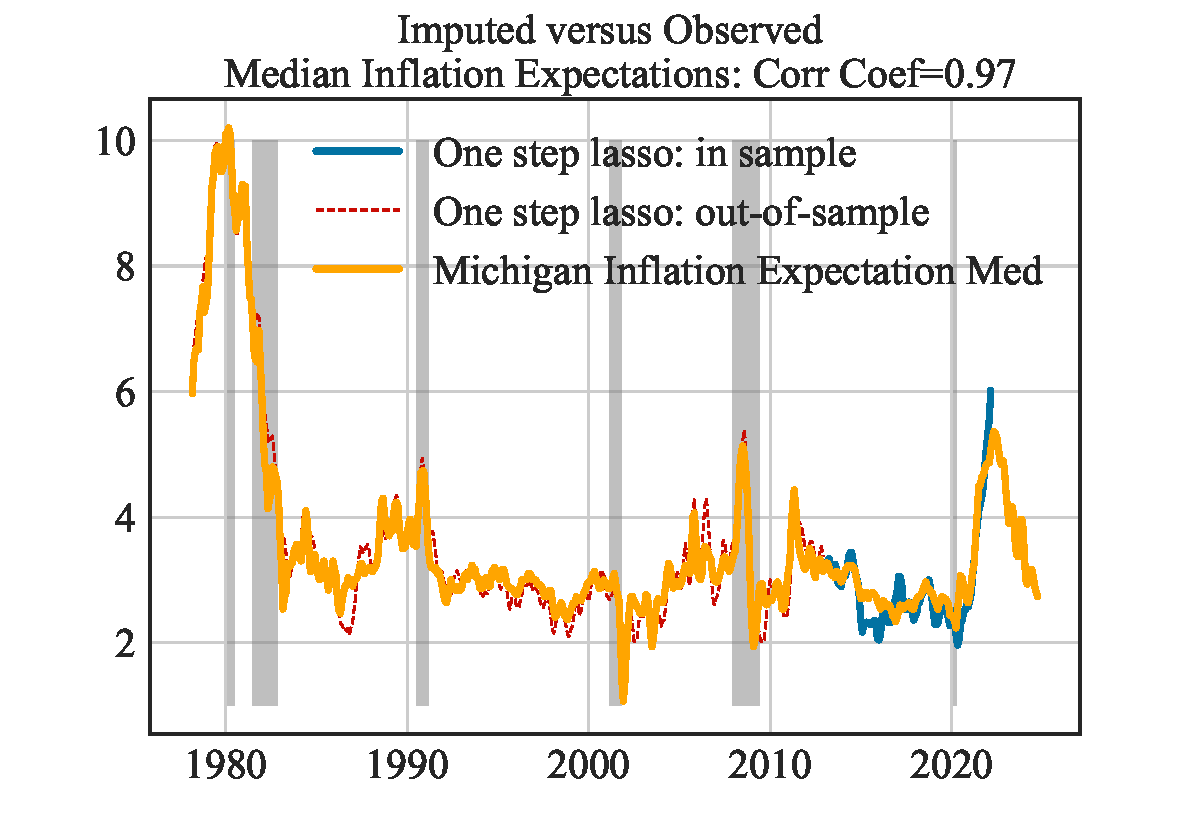
\includegraphics[width=0.49\linewidth]{Figures/imputed_comparison_inflation_msc_1step.pdf}  
    	\end{center}
    	
    	\begin{flushleft}Note: the figure plots the imputed beliefs from SCE regarding the percent chance the nationwide unemployment rate will be higher in the next year relative to the unemployment expectation index in MSC.\end{flushleft}
    \end{figure}



As a further validation of the imputation methodology across surveys, Figure \ref{fig:impute_cv_with_msc_ue} plots the imputed expectations in SCE regarding the median percent probability of nationwide unemployment rate to be higher, against the series of Michigan index regarding the direction of unemployment rate, which was observed for a much longer period. Again, in our in-sample Lasso imputation, we particularly exclude all Michigan indices regarding unemployment expectations to make it a fair test of the validity of our imputation methods. Because the SCE unemployment expectations are expressed as a percent probability while the MSC index is measured as the share of respondents expecting higher unemployment rates minus those expecting lower, we can not directly compare the imputation errors out-of-sample. We nevertheless show that the correlation between imputed expectations and the observed index in MSC is as high as 0.99. This suggests that our imputation method is able to do a great job of backcasting beliefs.   

 \begin{figure}[pt]
    	\caption{Imputed SCE versus Observed UE Expectations in MSC}
    	\label{fig:impute_cv_with_msc_ue}
    	\begin{center}
	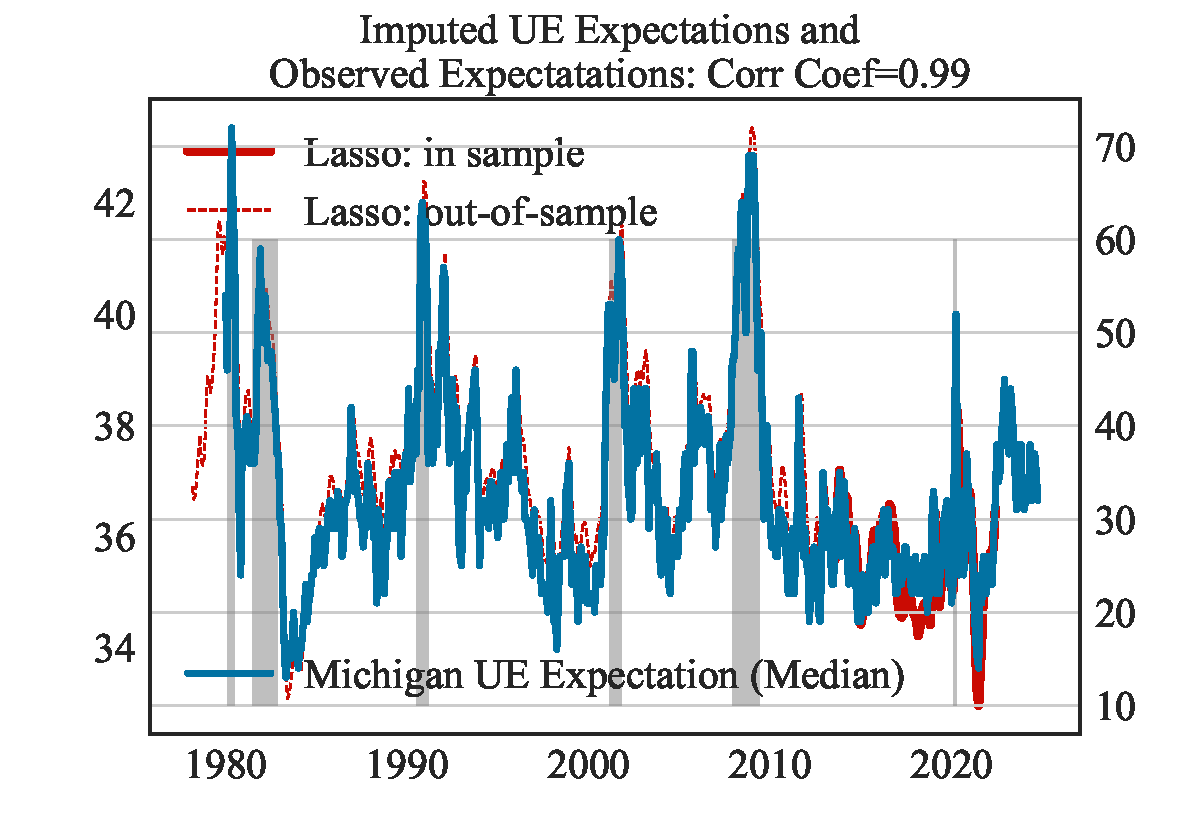
\includegraphics[width=0.6\linewidth]{Figures/imputed_comparison_ue_prob_msc_1step.pdf} 
    	\end{center}
    	
    	\begin{flushleft}Note: the figure plots the imputed beliefs from SCE regarding the percent chance the nationwide unemployment rate will be higher in the next year relative to the unemployment expectation index in MSC.\end{flushleft}
    \end{figure}

\subsubsection{Hyper-parameter tuning of the Lasso model using cross-validation}

 Figure \ref{fig:impute_cv} plots the model score, i.e. out-of-sample average MSE from k-fold samples, under various values of $\alpha$. 

      \begin{figure}[ht]
    	\caption{Model Selection using Cross-Validation}
    	\label{fig:impute_cv}
    	\begin{center}
	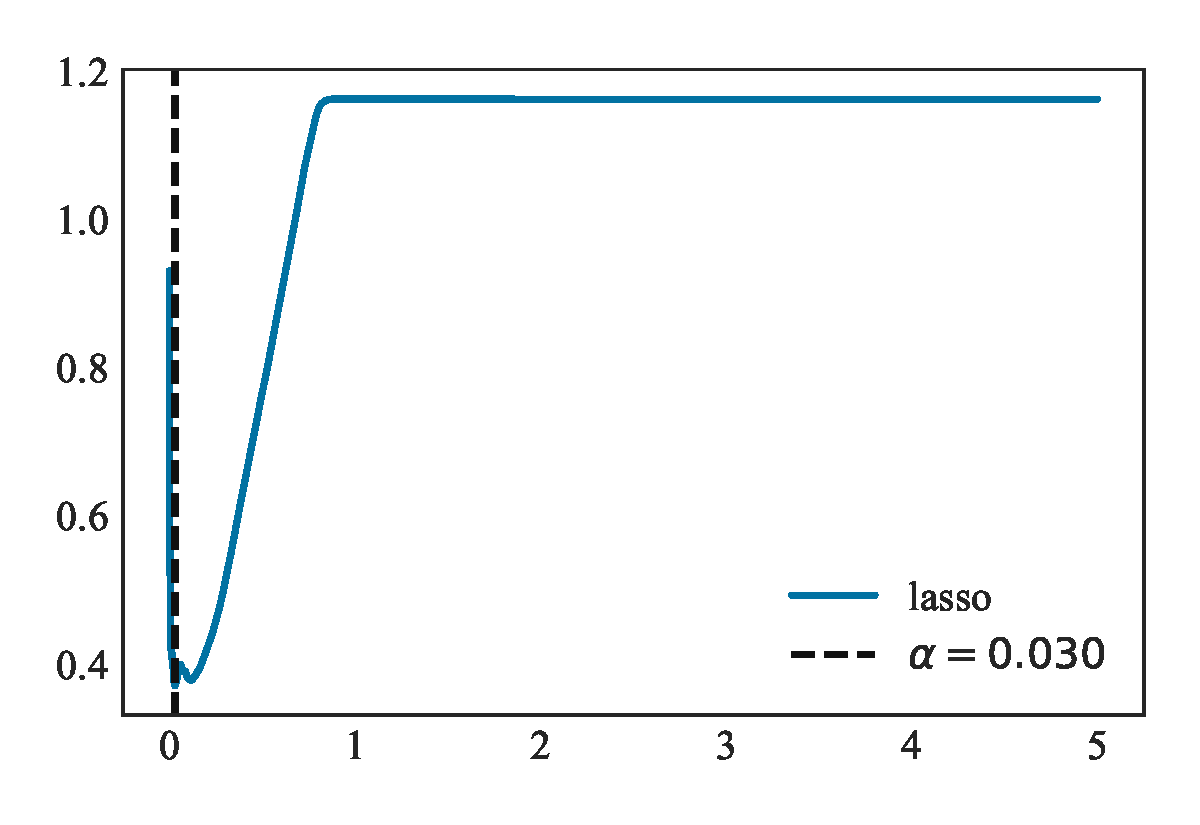
\includegraphics[width=0.48\linewidth]{Figures/unbounded_imputing_job_finding_cv.pdf} 
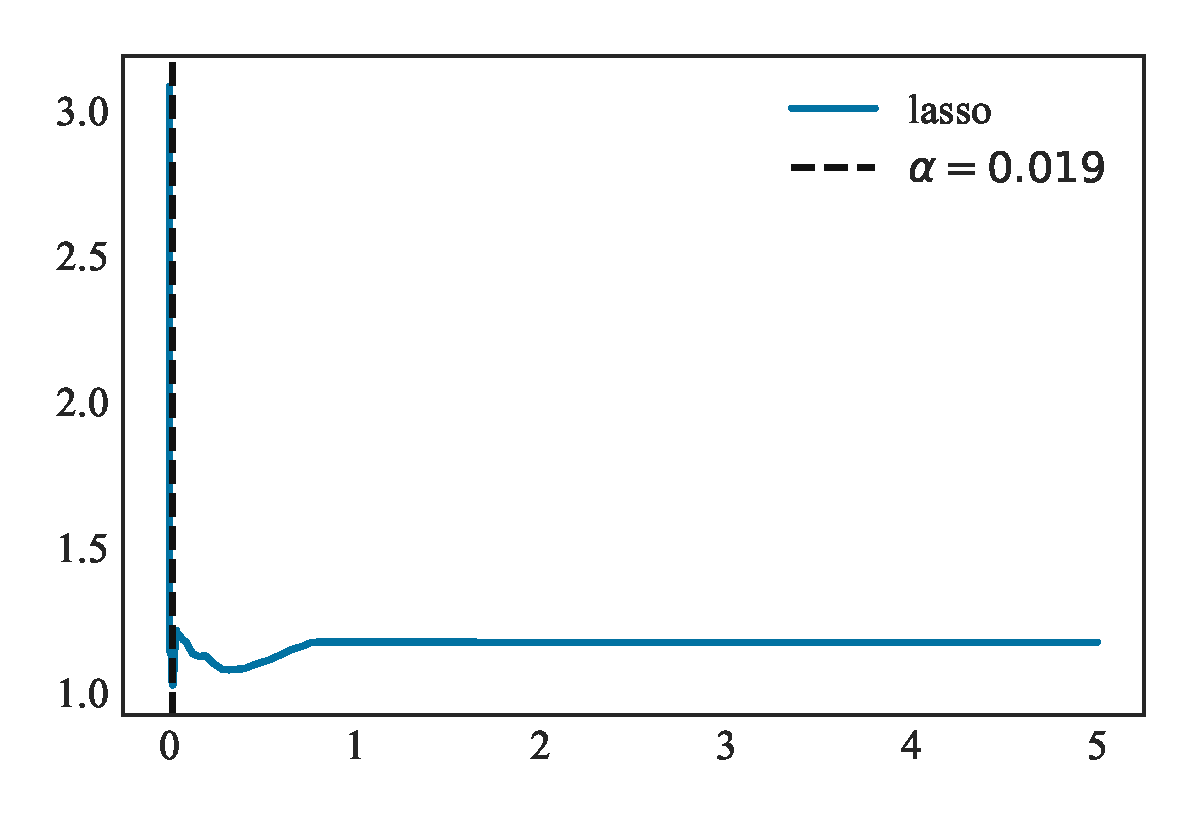
\includegraphics[width=0.48\linewidth]{Figures/unbounded_imputing_job_separation_cv.pdf} 
    	\end{center}
    
    	\begin{flushleft}Note: mean square error scores under different penalization parameter $\alpha$ of the Lasso model.\end{flushleft}
    \end{figure}
    
\subsubsection{Inclusion of the pandemic era}
\label{appendix:sensitivity_imputation}

Figure \ref{fig:imputed_JF_comparison_covid} compares the imputed job risk belief relied upon pre-2020 sample as the in-sample of Lasso model with one relied on an extended sample covering the Covid era (2020-2022). The gap between the two series reveals a possible structural break in the relationship between job perceptions and other household expectations and macroeconomic conditions. However, such a different choice of in-sample period of the belief imputation does not significantly alter the patterns of the imputed out-of-sample job beliefs. The major exception was the job separation perceptions in the early 1980s.  

\begin{figure}[pt]
    \centering
    \caption{Imputing Beliefs Including or Excluding Covid Era}\label{fig:imputed_JF_comparison_covid}
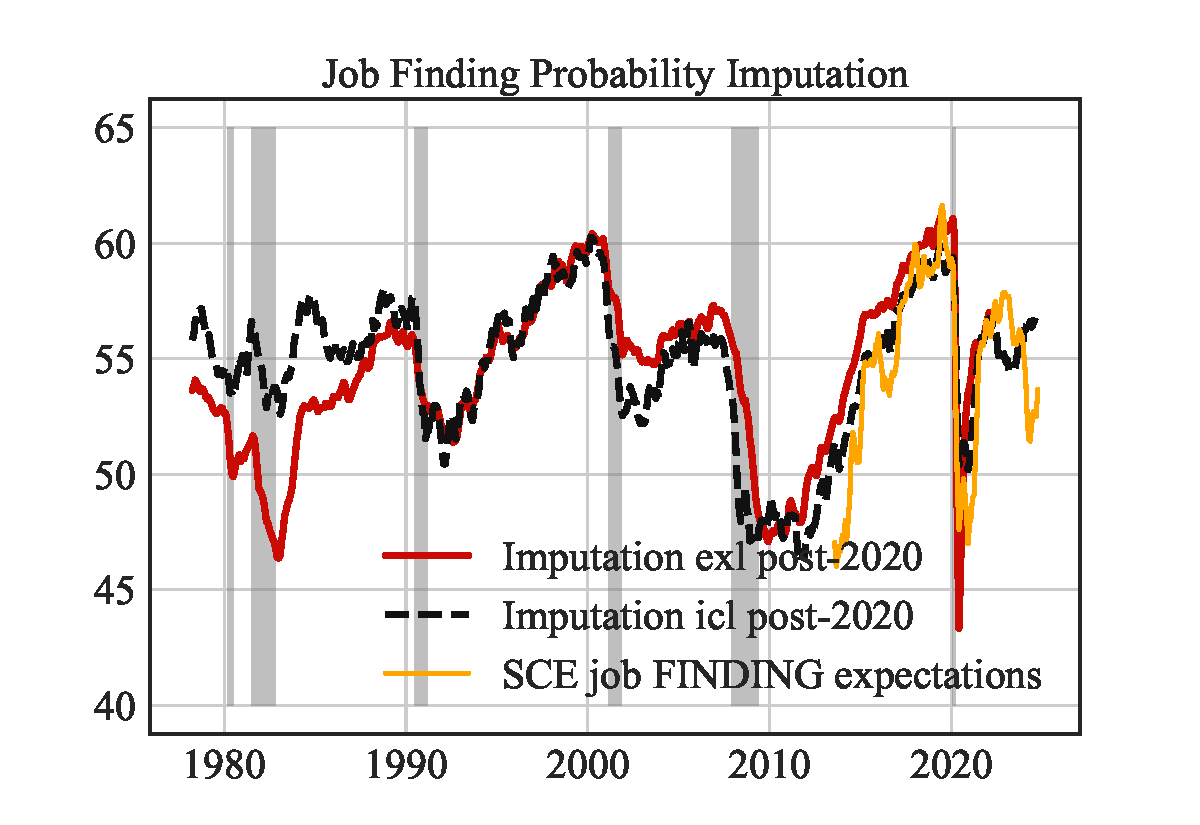
\includegraphics[width=0.7\linewidth]{Figures/imputed_JF_comparison_covid.pdf} 
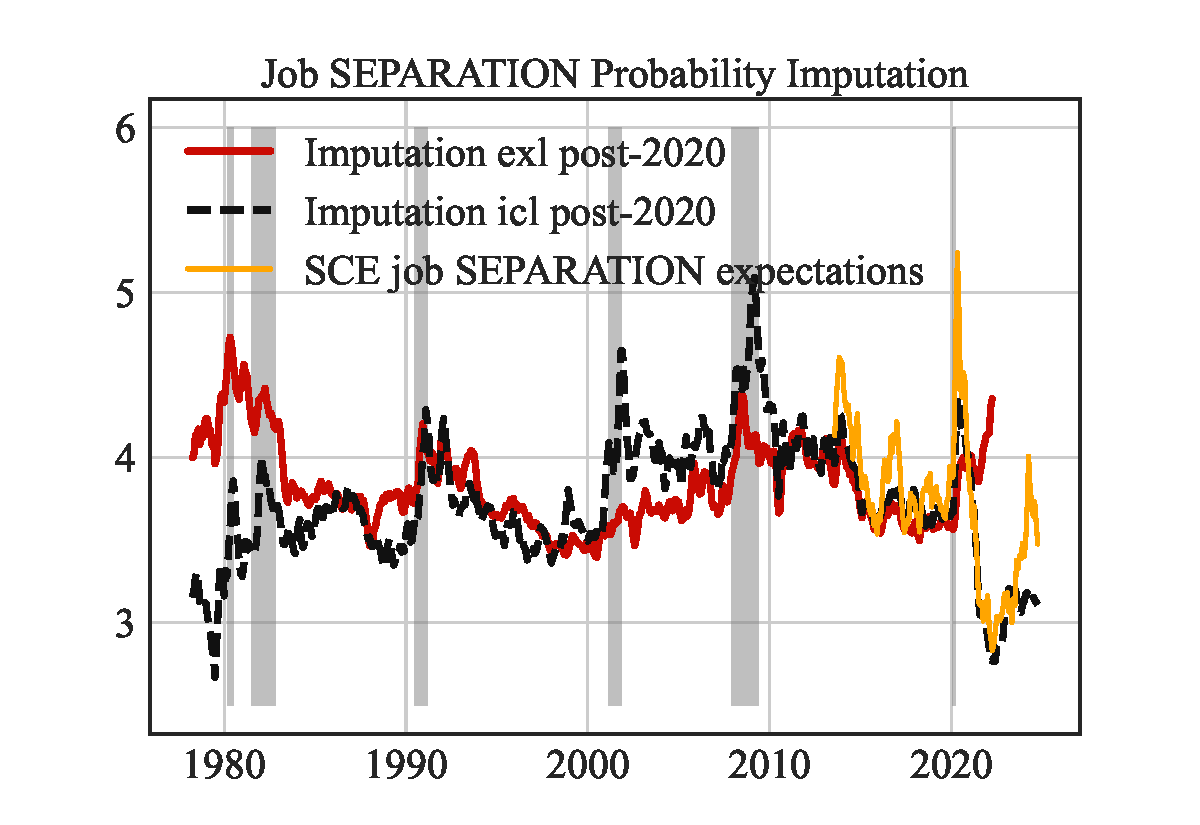
\includegraphics[width=0.7\linewidth]{Figures/imputed_JS_comparison_covid.pdf} 
\end{figure}

\subsubsection{Selected covariates of perceived risks}
\label{appendix: covariates_perceived_risks}

Figure \ref{fig:vars_rank} report the 10 most important variables selected from the Lasso model of imputation of perceived job risks, ranked by the absolute value of their estimated coefficients associated with the normalized value of each variable.  

    \begin{figure}[ht]
    	\caption{Selected variables of Lasso model of perceived job risks}
    	\label{fig:vars_rank}
    	\begin{center}
	\adjustimage{max size={0.48\linewidth}}{Figures/covariates_rank_job_finding.pdf} 
 	\adjustimage{max size={0.48\linewidth}}{Figures/covariates_rank_job_separation.pdf} 

    	\end{center}
    	
    	\begin{flushleft}\footnotesize{Note: selected variables ranked by the absolute value of their estimated coefficients in the Lasso imputation model for perceived job finding (left) and separation (right). The in-sample is between 2013-2020. UERate: real-time unemployment rate. Durrn\_gt\_all: good time to buy durables. Pexp\_f\_all: expecting better personal finance one year from now. Bus12\_f\_all: better nationwide business conditions a year from now. Px1\_15p\_all: expected inflation above 15 percent. Vehrn\_gt\_all: good time to buy vehicles. ptrd\_bb\_all: better off financially a year ago and better off a year from now. bago\_s\_all: same business conditions compared to a year ago. Pagorn\_hp\_all: worse financial situation than a year ago due to higher prices. Ptrd\_ss\_all: same personal finance compared to a year ago and will be the same a year from now. Pexp\_u\_all: worse personal finance one year from now. Newsrn\_u\_eng\_all: heard unfavorable news about the energy crisis. Newsrn\_u\_stk\_all: heard about unfavorable news regarding the stock market. Vehrn\_fb\_all: a bad time to buy vehicles due to uncertain future. Px1\_dkup\_all: do not know about future inflation. Newsrn\_u\_dem\_all: heard unfavorable news about lower consumer demand. INF\_Y2Y: real-time annual realized inflation rate. Bago\_f\_all: better business conditions compared to a year ago. Pagorn\_hd\_all: worse personal finance due to higher debt.}  \end{flushleft}
    \end{figure}

   \begin{figure}[ht]
    	\caption{Imputed job finding rate and realizations}
    	\label{fig:impute_comparison_1step}
    	\begin{center}
	\adjustimage{max size={0.7\linewidth}}{Figures/unbounded_imputed_comparison_1step_job_finding.pdf} \\
 	\adjustimage{max size={0.7\linewidth}}{Figures/unbounded_imputed_comparison_1step_job_separation.pdf}
    	\end{center}
    	\begin{flushleft}\footnotesize{Note: imputed perceived risks in the sample (2013-2022) and out-of-sample (1980-2013) compared to realized job flow rates.} \end{flushleft}
    \end{figure}


\subsubsection{Imputed beliefs by education group}

Figure \ref{fig:impute_by_education} plots the in-sample fitted and out-of-sample imputed perceptions of the job finding and separations rates for low, middle, and high education groups, versus the realized rates for each group. 

 \begin{figure}[pt]
    	\caption{Imputed beliefs by education}
    	\label{fig:impute_by_education}
    	\begin{center}
	\adjustimage{max size={0.43\linewidth}}{Figures/imputed_comparison_JF_LowEdu_1step.pdf}  
 	\adjustimage{max size={0.43\linewidth}}{Figures/imputed_comparison_JS_LowEdu_1step.pdf}  \\
 	\adjustimage{max size={0.43\linewidth}}{Figures/imputed_comparison_JF_MidEdu_1step.pdf} 	\adjustimage{max size={0.43\linewidth}}{Figures/imputed_comparison_JS_MidEdu_1step.pdf} \\
  	\adjustimage{max size={0.43\linewidth}}{Figures/imputed_comparison_JF_HighEdu_1step.pdf} 
    	\adjustimage{max size={0.43\linewidth}}{Figures/imputed_comparison_JS_HighEdu_1step.pdf} 
    	\end{center}
    	
    	\begin{flushleft}\footnotesize {Note: these figures plot the imputed perceived job separation and finding rates by low, middle and high educations, respectively, using the same methodology and the education-specific expectations in MSC.}\end{flushleft}
    \end{figure}

   

\subsection{Additional results with forecast errors}
\label{appendix:fe_results_more}

    The upper panel in Figure \ref{fig:forecast_errors} plots the FEs using two alternative series as realizations of job findings. During the majority of times in the sample, FEs lie in the negative domains, suggesting that on average, household beliefs underpredicted the realization of job-findings. This is consistent with the observation in Figure \ref{fig:impute_comparison_1step} that the imputed beliefs are below the realization most of the time. The periods with notable exceptions were the 1981-1982 recession and the Great Recession.
    
   
\begin{figure}[ht]
\caption{Forecast errors of job-finding and separation expectations}
\label{fig:forecast_errors}    
     	\begin{center}
 		%\adjustimage{max size={0.68\linewidth}}{Figures/forecast_errors.pdf} \\
 			\adjustimage{max size={0.8\linewidth}}{Figures/forecast_errors_size.pdf} %\\
    	\adjustimage{max size={0.8\linewidth}}{Figures/forecast_errors_size_job_separation.pdf} \\
 \end{center}
 \begin{flushleft}\footnotesize{Note: the absolute value of forecast errors of job finding and separation rates, defined as the difference both imputed/or observed perceived risk and the realized job transition rates.} \end{flushleft}
\end{figure}
    
    The lower panel plots the size of (absolute values) of the FEs. The size of FEs seemed to dramatically drop during recessions, compared to normal times. Some research has found that information-rigidity is counter-cyclical.\footnote{See \cite{coibion2015information} for the evidence with inflation expectations.}


\subsection{Additional evidence for the belief distortions over business cycles}

Instead of calculating peak-to-trough values of job risks as in Figure \ref{fig:bus_cycle_stats},  Figure \ref{fig:bus_cycle_stats_av} plots the average job finding/separation rates in normal times versus recessions and their average ratios, which show largely similar business cycle patterns of realized transition rates, risk forecasts and perceived job risks. 

\begin{figure}[pt] 
\centering 
	\caption{Business Cycle Patterns of Risks and Perceptions: Normal Times versus Recessions} 
	\label{fig:bus_cycle_stats_av}
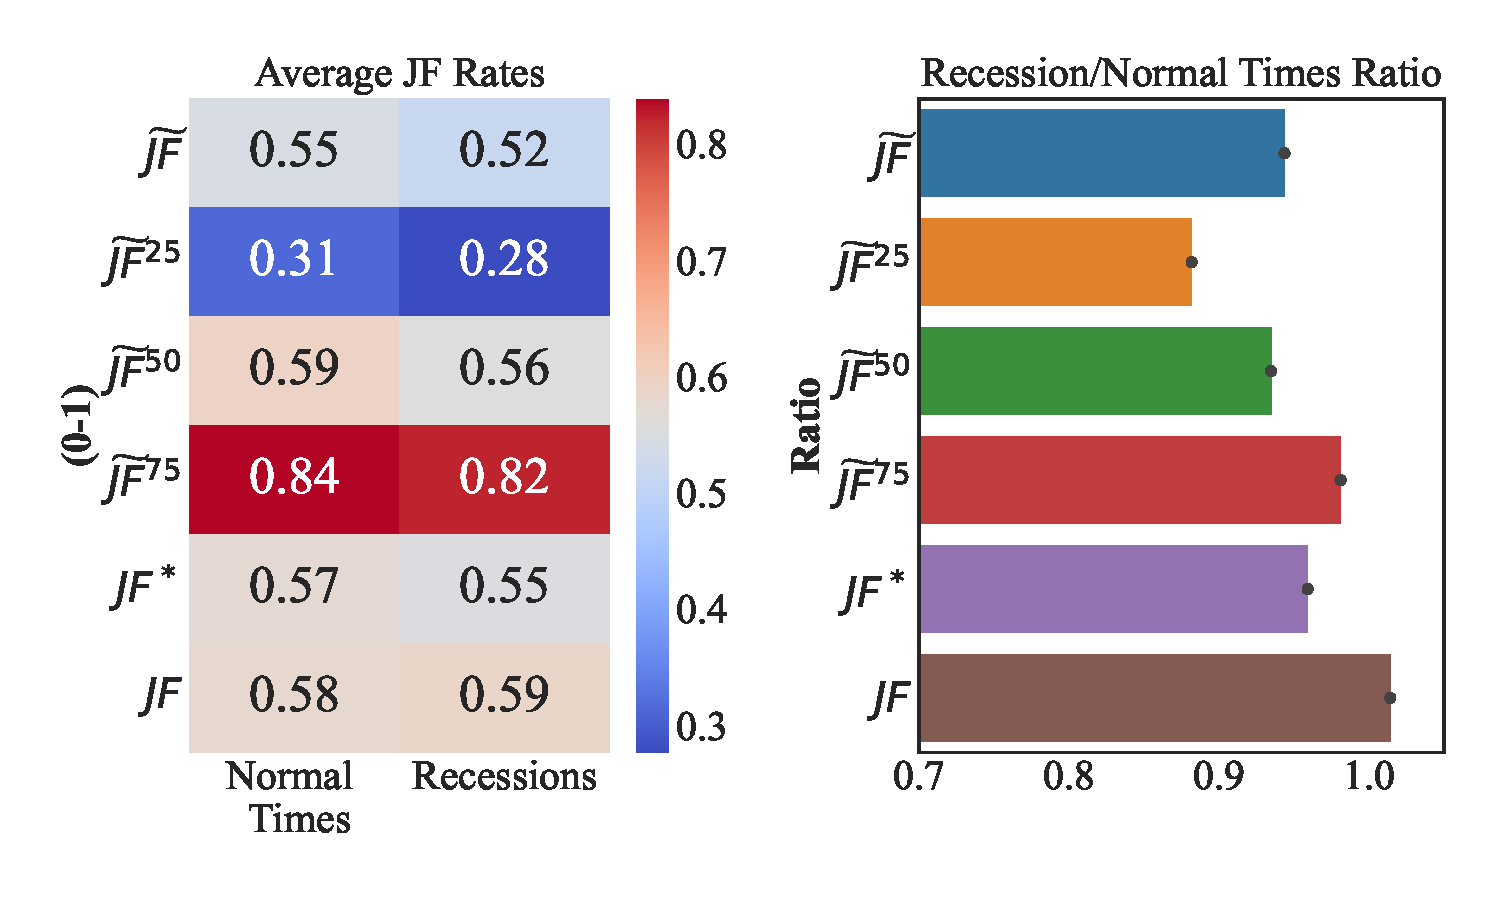
\includegraphics[width=0.8\linewidth]{Figures/business_cycle_JF_stats.pdf} \\
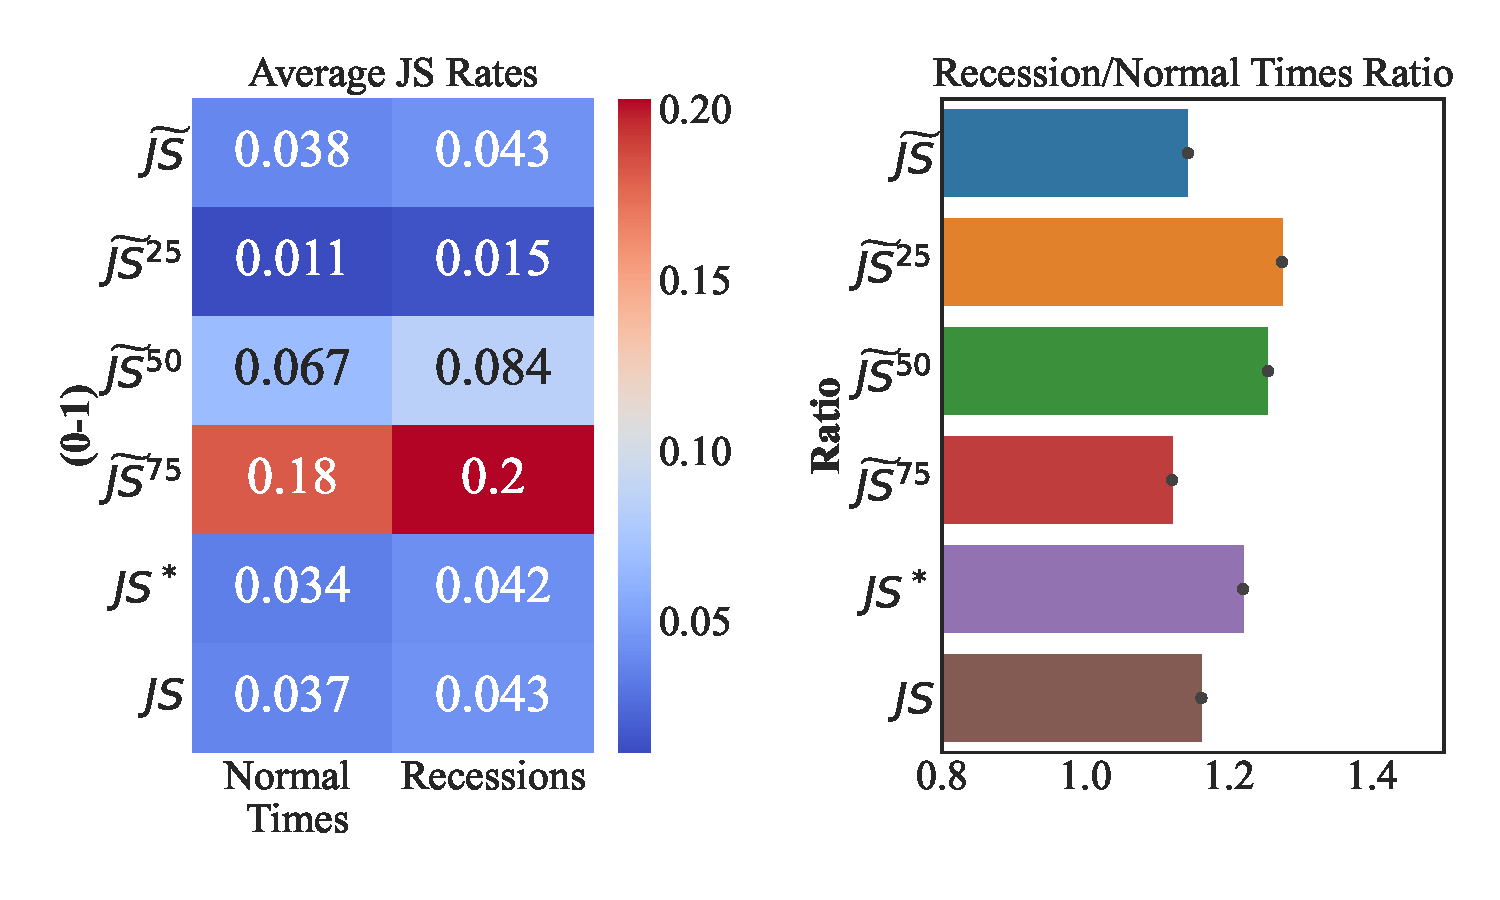
\includegraphics[width=0.8\linewidth]{Figures/business_cycle_JS_stats.pdf} \\
    	\begin{flushleft}\footnotesize {Note: The left tables report the average perceived job risks, perceived job risks at different quantiles, real-time job risks, and realized job transition rates in normal times and NBER-labeled recessions. The right figures plot the ratio of these rates between recessions and normal times. The sample period is 1990-2024.} \end{flushleft}
\end{figure}



\section{Additional Model Results}
\label{appendix:model_results}

\input{model.tex}


\subsection{Details of the model experiments}

\subsubsection{Baseline model at the quarterly frequency}

The model experiments in Figure \ref{fig:pe_decompose_sub_obj} are based on directly estimated shocks to $JF$/$JS$, $\widetilde{JF}/\widetilde{JS}$ and ${JF}^*/{JS}^*$. To obtain such shocks, we estimate, respectively, a quarterly AR(1) model of each one of these sequences in the sample period up to the 2020 Q1. The predicted residuals are the estimated shocks to realized rates, beliefs, and rational job risk, which are plotted in Figure \ref{fig:shocks_from_data}. 

\begin{figure}[pt]
    \centering
    \caption{Shocks to realized job transitions, perceptions and rational forecasts}
    \label{fig:shocks_from_data} 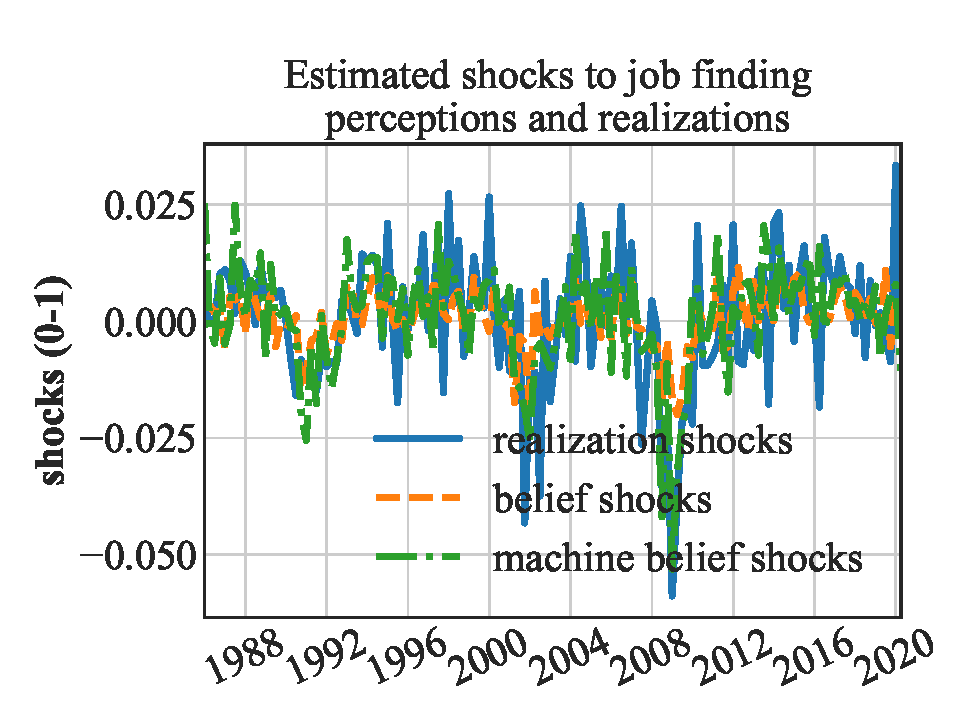
\includegraphics[width=0.45\linewidth]{Figures/estimated_shocks_job_finding.pdf}
    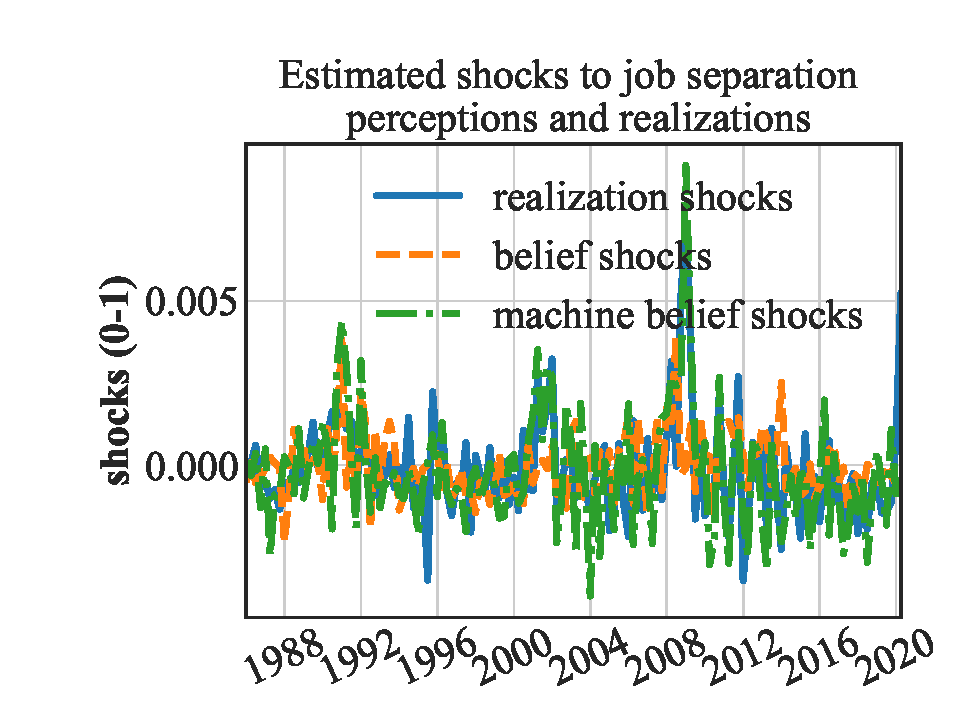
\includegraphics[width=0.45\linewidth]{Figures/estimated_shocks_job_separation.pdf}
\begin{flushleft}\footnotesize {Note: The figure plots the estimated shocks used for the experiments in Figure \ref{fig:pe_decompose_sub_obj}, based on an estimation of a quarterly AR(1) model on demeaned $JS_{t}\& JF_t$, $\widetilde{JS}_t \& \widetilde{JF}_t$, and $JS^{*}_t \& JF^{*}_t$. The sample period is between 1987 and 2020.} \end{flushleft}
\end{figure}


%\begin{figure}[pt]
%    \centering
%    \caption{Unemployment rate dynamics implied by the time paths of job finding and separation rates}
    %\label{fig:urate_model_data} 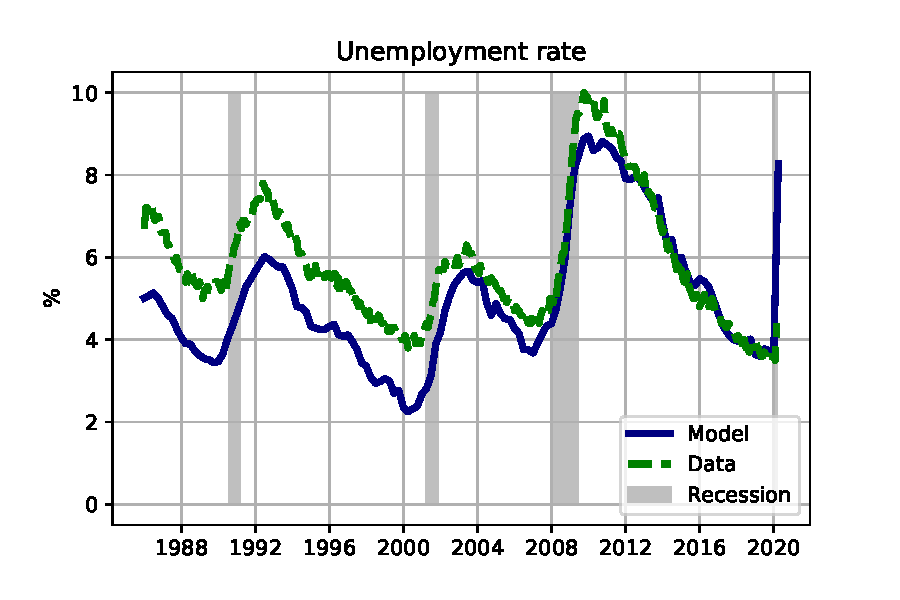
\includegraphics[width=0.6\linewidth]{Figures/unemployment_rate_model_data.pdf}
%\begin{flushleft}\footnotesize {Note: The figure plots the simulated unemployment rate path based on the estimated shocks to realized $JS$ and $JF$ rates for the period 1988-2020. They are used for the experiments in Figure \ref{fig:pe_decompose_sub_obj}.} \end{flushleft}
%\end{figure}

Figure \ref{appendix_pe_decompose_sub_obj_educ} complements Figure \ref{fig:pe_decompose_sub_obj_educ} by showing the education-specific consumption aggregation fluctuations due to job separation and finding risks, separately. 

  \begin{figure}
        \centering
          \caption{Consumption Fluctuations due to JS and JF Risks: by Education}
\label{appendix_pe_decompose_sub_obj_educ}
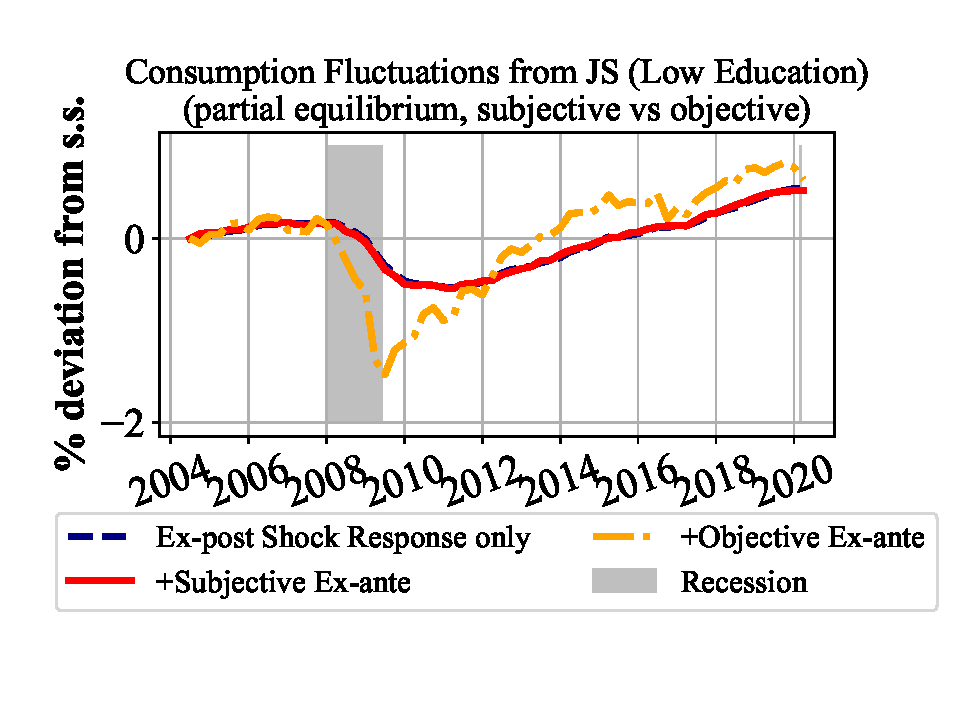
\includegraphics[width=0.4\linewidth]{Figures/consumption_pe_JS_deviation_machine_as_rational_LowEdu.pdf}
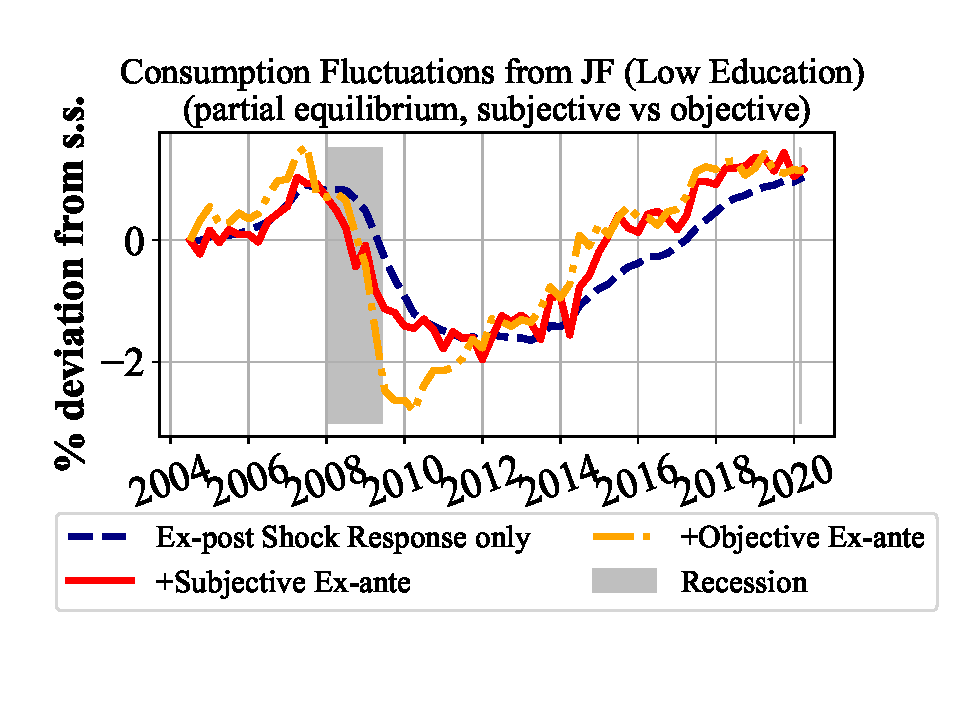
\includegraphics[width=0.4\linewidth]{Figures/consumption_pe_JF_deviation_machine_as_rational_LowEdu.pdf}
%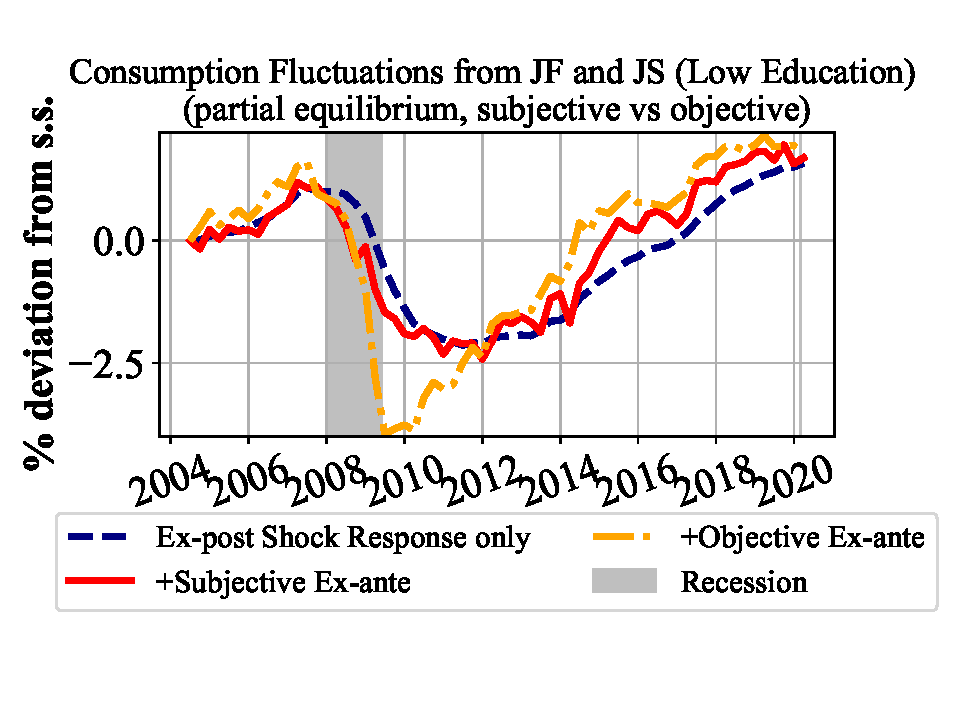
\includegraphics[width=0.6\linewidth]{Figures/consumption_pe_JS_JF_deviation_machine_as_rational_LowEdu.pdf} 
\\
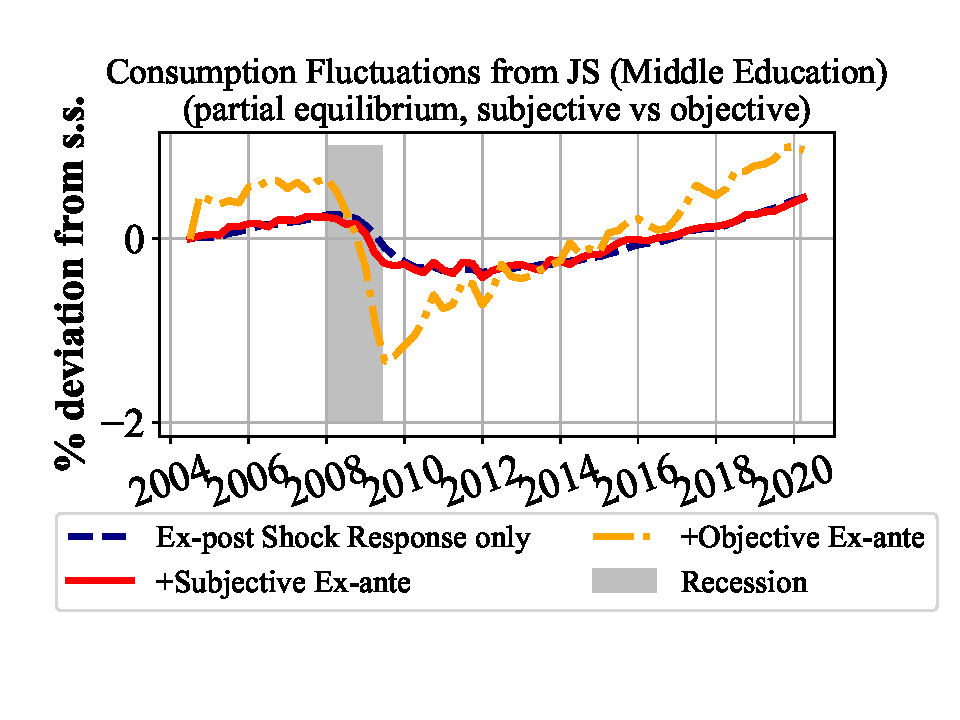
\includegraphics[width=0.4\linewidth]{Figures/consumption_pe_JS_deviation_machine_as_rational_MidEdu.pdf}
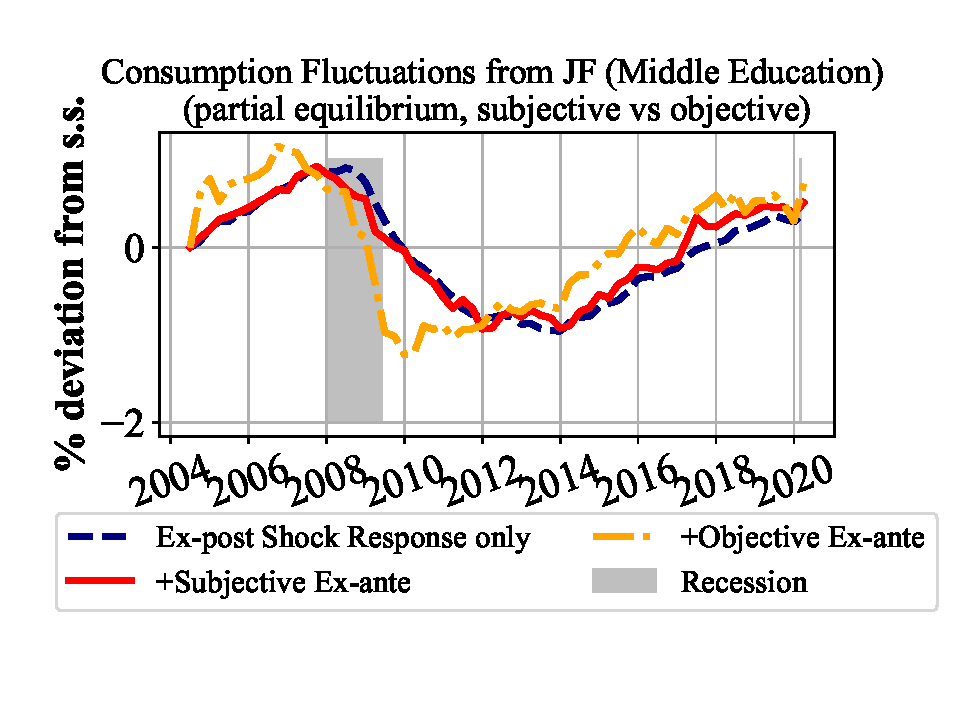
\includegraphics[width=0.4\linewidth]{Figures/consumption_pe_JF_deviation_machine_as_rational_MidEdu.pdf}
%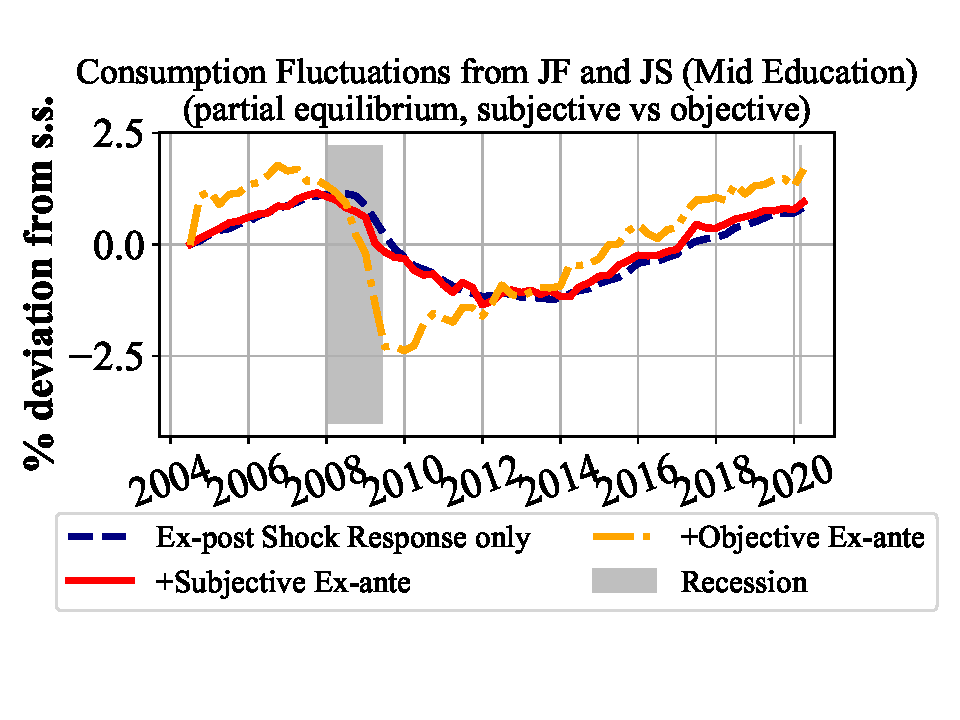
\includegraphics[width=0.6\linewidth]{Figures/consumption_pe_JS_JF_deviation_machine_as_rational_MidEdu.pdf}
\\

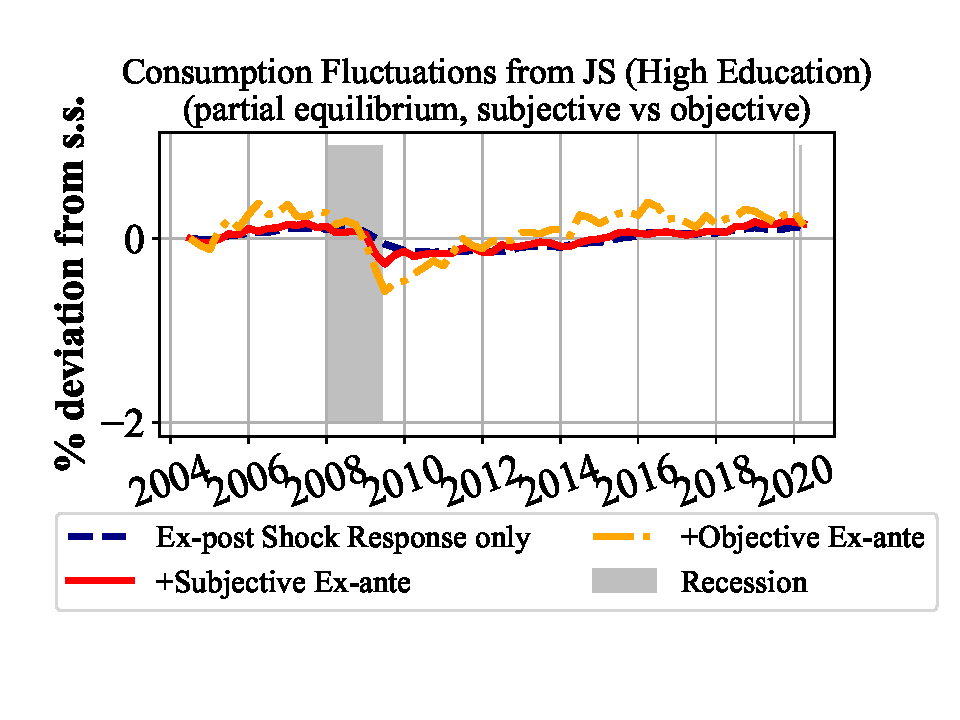
\includegraphics[width=0.4\linewidth]{Figures/consumption_pe_JS_deviation_machine_as_rational_HighEdu.pdf}
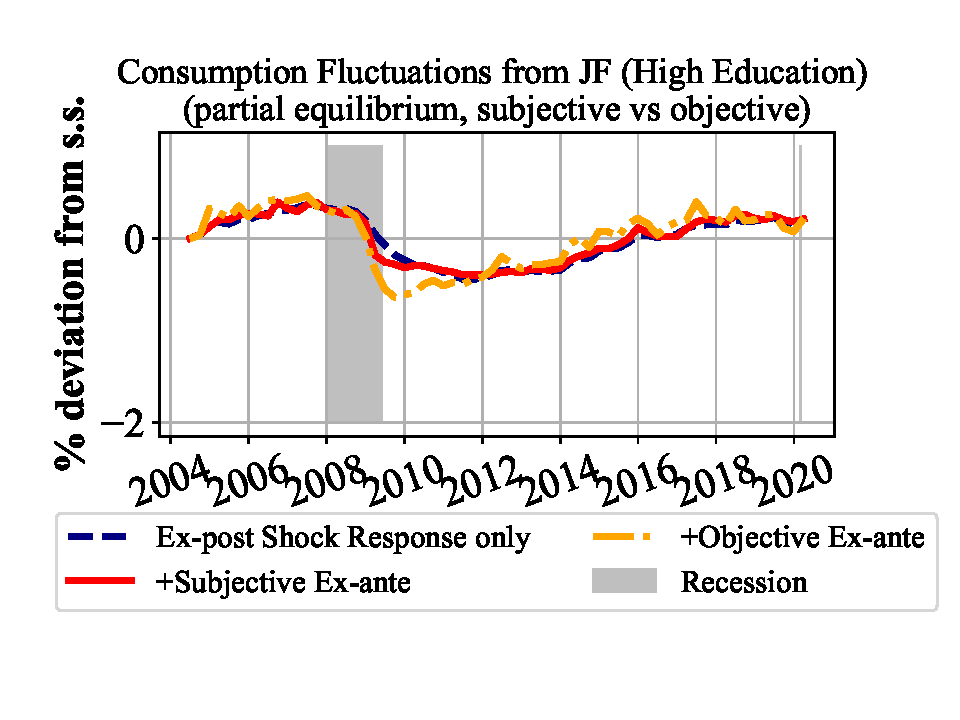
\includegraphics[width=0.4\linewidth]{Figures/consumption_pe_JF_deviation_machine_as_rational_HighEdu.pdf}
%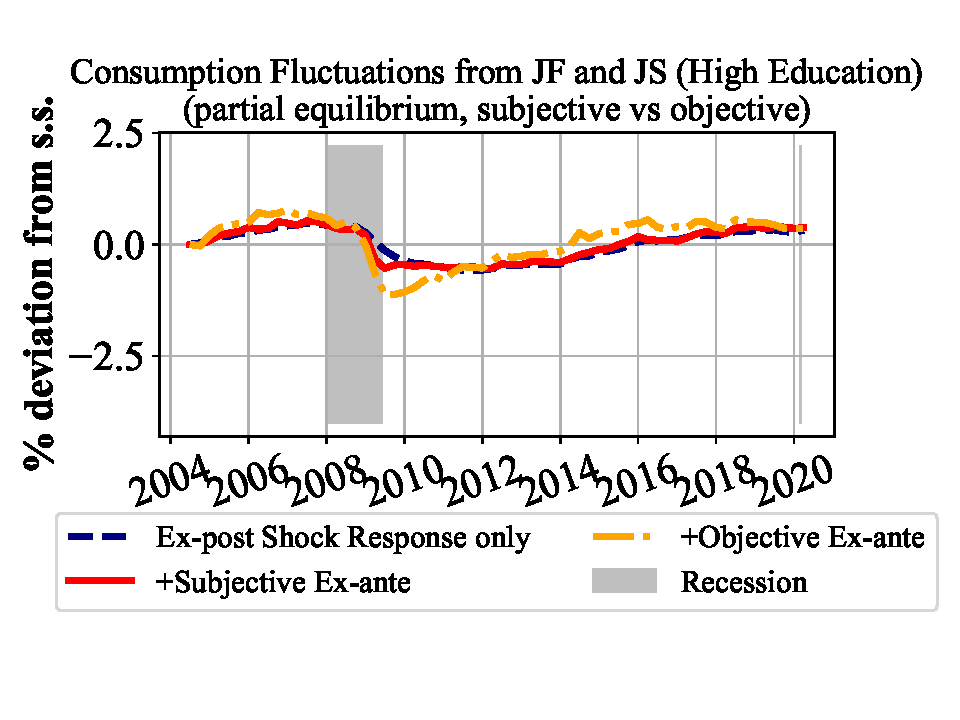
\includegraphics[width=0.6\linewidth]{Figures/consumption_pe_JS_JF_deviation_machine_as_rational_HighEdu.pdf}
      \begin{flushleft}\footnotesize {Note: The figure compares for each education group their partial-equilibrium aggregate consumption deviations from its steady state simulated based on empirically estimated shocks to perceived job risk (subjective) and the real-time forecast risk (objective), in addition to the ex-post response to shocks to the realized job transition rates.} \end{flushleft}
    \end{figure}


\begin{center}\renewcommand{\arraystretch}{1.5}
\begin{table}
\centering
\caption{Household Calibration}\label{table:Calibration}
\makebox[\textwidth]{\begin{tabular}{|c|ccl|c|}
\hline
Description                     & \multicolumn{1}{c}{Parameter} & Value & \multicolumn{2}{c|}{Source/Target }\\ \hline
CRRA & \multicolumn{1}{c}{CRRA} & 2 & \multicolumn{2}{c|}{Standard} \\
Real Interest Rate                 & \multicolumn{1}{c}{$r$} & $1.03^{.25} - 1$ & \multicolumn{2}{c|}{ 3\% annualized real rate} \\
Probability of Death       & \multicolumn{1}{c}{$D$} & 0.00625 & \multicolumn{2}{c|}{\cite{carroll2017distribution}} \\
 \hline


UI replacement rate& \multicolumn{1}{c}{$\gamma$} & 0.5 & \multicolumn{2}{c|}{ 50$\%$ income drop at unemployment} \\
%Non UI income parameter 1 &  \multicolumn{1}{c}{$\gamma_{1}$} & 0.76 & \multicolumn{2}{c|}{ \cite{kekre2023unemployment} }\\
%Non UI income parameter 2 &  \multicolumn{1}{c}{$\gamma_{2}$} & 0.55 & \multicolumn{2}{c|}{\cite{kekre2023unemployment}} \\
%Gov. transfers &  \multicolumn{1}{c}{$T_{s}$} & 0.091 & \multicolumn{2}{c|}{\begin{footnotesize} $\frac{\text{SNAPS and Soc. Security Inc}}{\text{Pre Job Loss Income}} = .13$ \end{footnotesize}} \\
Std Dev of Log Permanent Shock  & \multicolumn{1}{c}{$\sigma_{\psi}$} & 0.06 & \multicolumn{2}{c|}{\cite{carroll2017distribution}} \\
Std Dev of Log Transitory Shock & \multicolumn{1}{c}{$\sigma_{\theta}$} & 0.2 & \multicolumn{2}{c|}{\cite{carroll2017distribution}} \\  \hline

Steady state Job Finding Rate & \multicolumn{1}{c}{$JF$} & 0.58 & \multicolumn{2}{c|}{CPS} \\ 
Steady state Job Separation Rate& \multicolumn{1}{c}{$JS$} & 0.070 & \multicolumn{2}{c|}{steady state unemployment rate=0.05} \\  \hline
Discount Factor & \multicolumn{1}{c}{$\beta$} &  0.976 & \multicolumn{2}{c|}{Quarterly MPC = 0.16} \\  \hline
\end{tabular}}
\end{table}
\end{center}



\subsubsection{Alternative model experiment at monthly frequency}

In this section, we report results from the baseline model experiments with a monthly version of the model with several modifications, which is calibrated similarly to \cite{kekre2023unemployment}. Since working with a quarterly model inevitably involves time-aggregation of monthly job flow rates and their belief counterparts, we see a monthly model as more robust to our assumptions on the time-aggregation. In particular, we replace the permanent wage component with a persistent component with a monthly AR(1) coefficient of 0.997, and a standard deviation of the shock of 0.057. We use steady-state monthly job finding rate to be 0.2517, the sample average from CPS before Covid era. 

Modifying the quarterly model assumption, we also assume that employment-to-unemployment transition is entirely driven by job separations, e.g.  $p(n_{i,t+1}=u|n_{i,t}=e) = JS_{t})$. We set its average to be 0.017. The discount factor beta is estimated to yield a quarterly MPC of 0.21, a la \cite{kekre2023unemployment}.  Figure \ref{fig:pe_decompose_sub_obj_monthly} shows the results with homogeneous workers, and Figure \ref{fig:pe_decompose_sub_obj_educ_monthly} shows that with heterogeneous risks by education.

\begin{figure}[ht]
    \centering
    \caption{\textbf{Monthly} Consumption Fluctuations due to Unemployment Risks}
    \label{fig:pe_decompose_sub_obj_monthly}

    \begin{subfigure}{0.32\linewidth}
         \caption*{Job separation}
        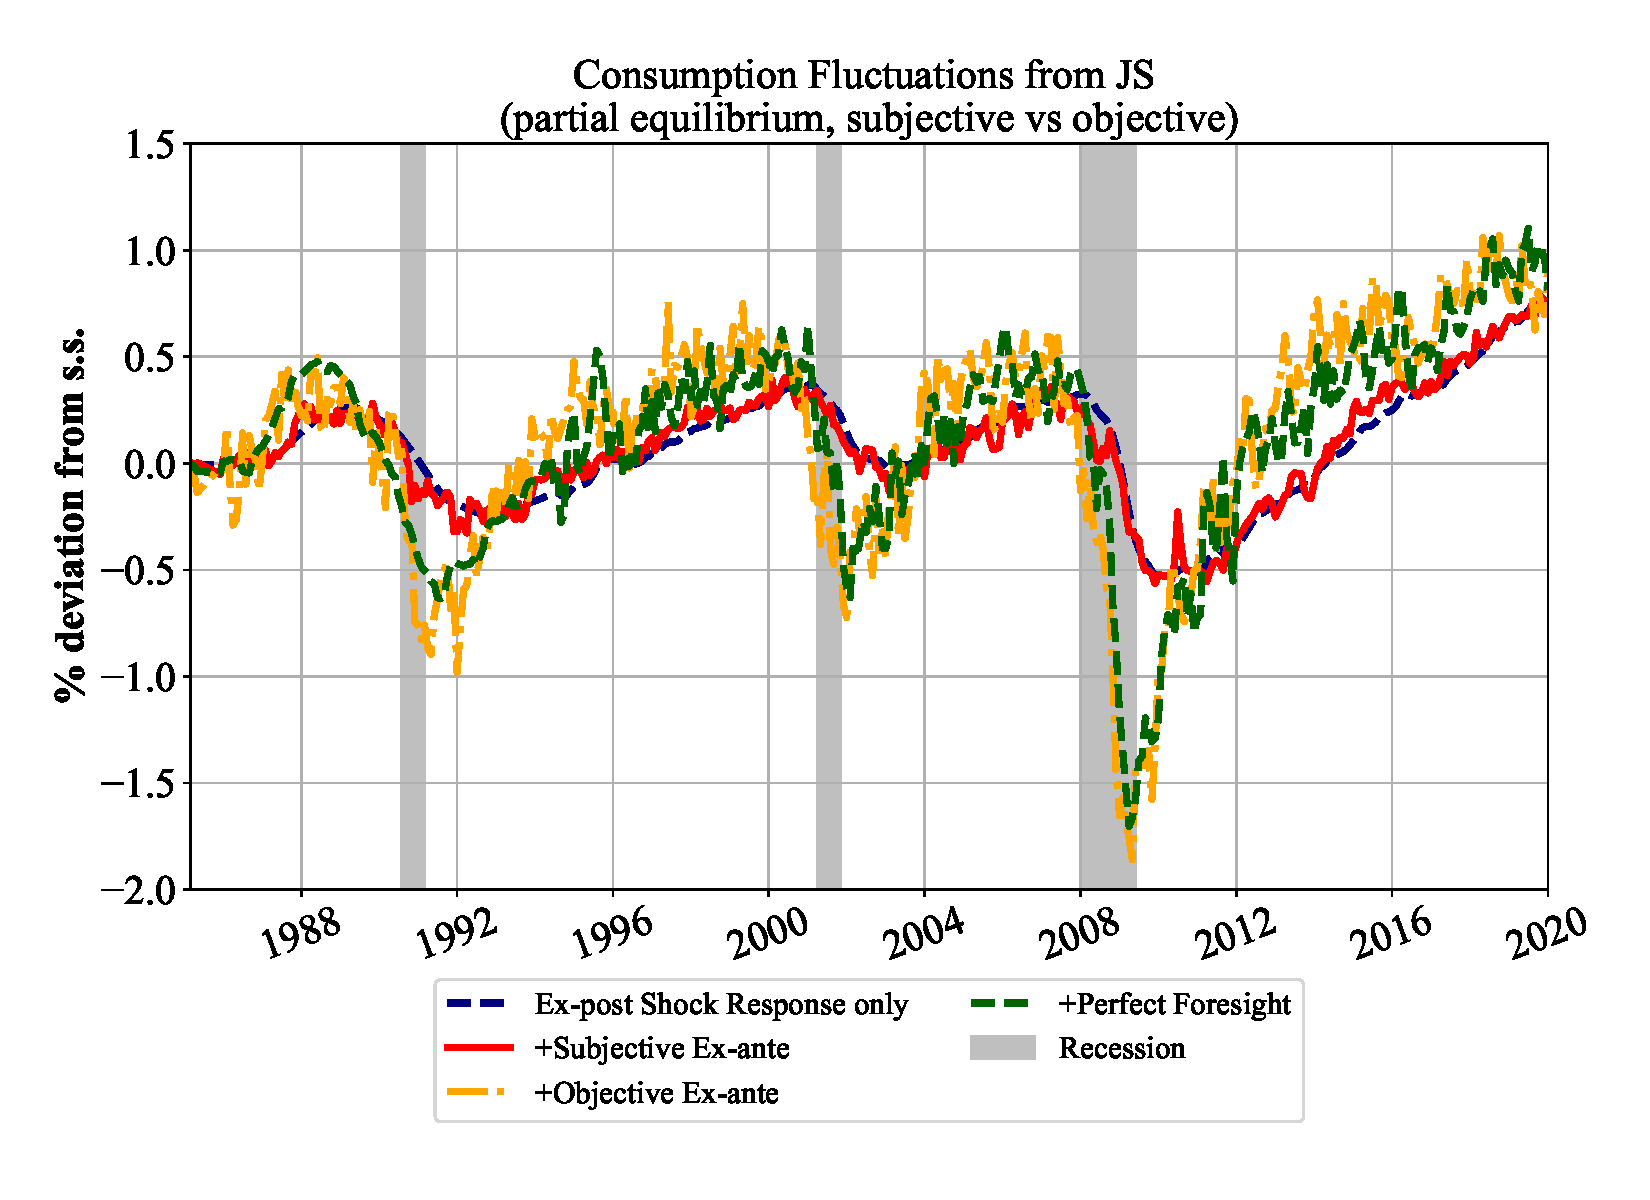
\includegraphics[width=\linewidth]{Figures/consumption_pe_JS_deviation_machine_as_rational_monthly.pdf}
   
    \end{subfigure}
    \hfill
    \begin{subfigure}{0.32\linewidth}
         \caption*{Job finding}
        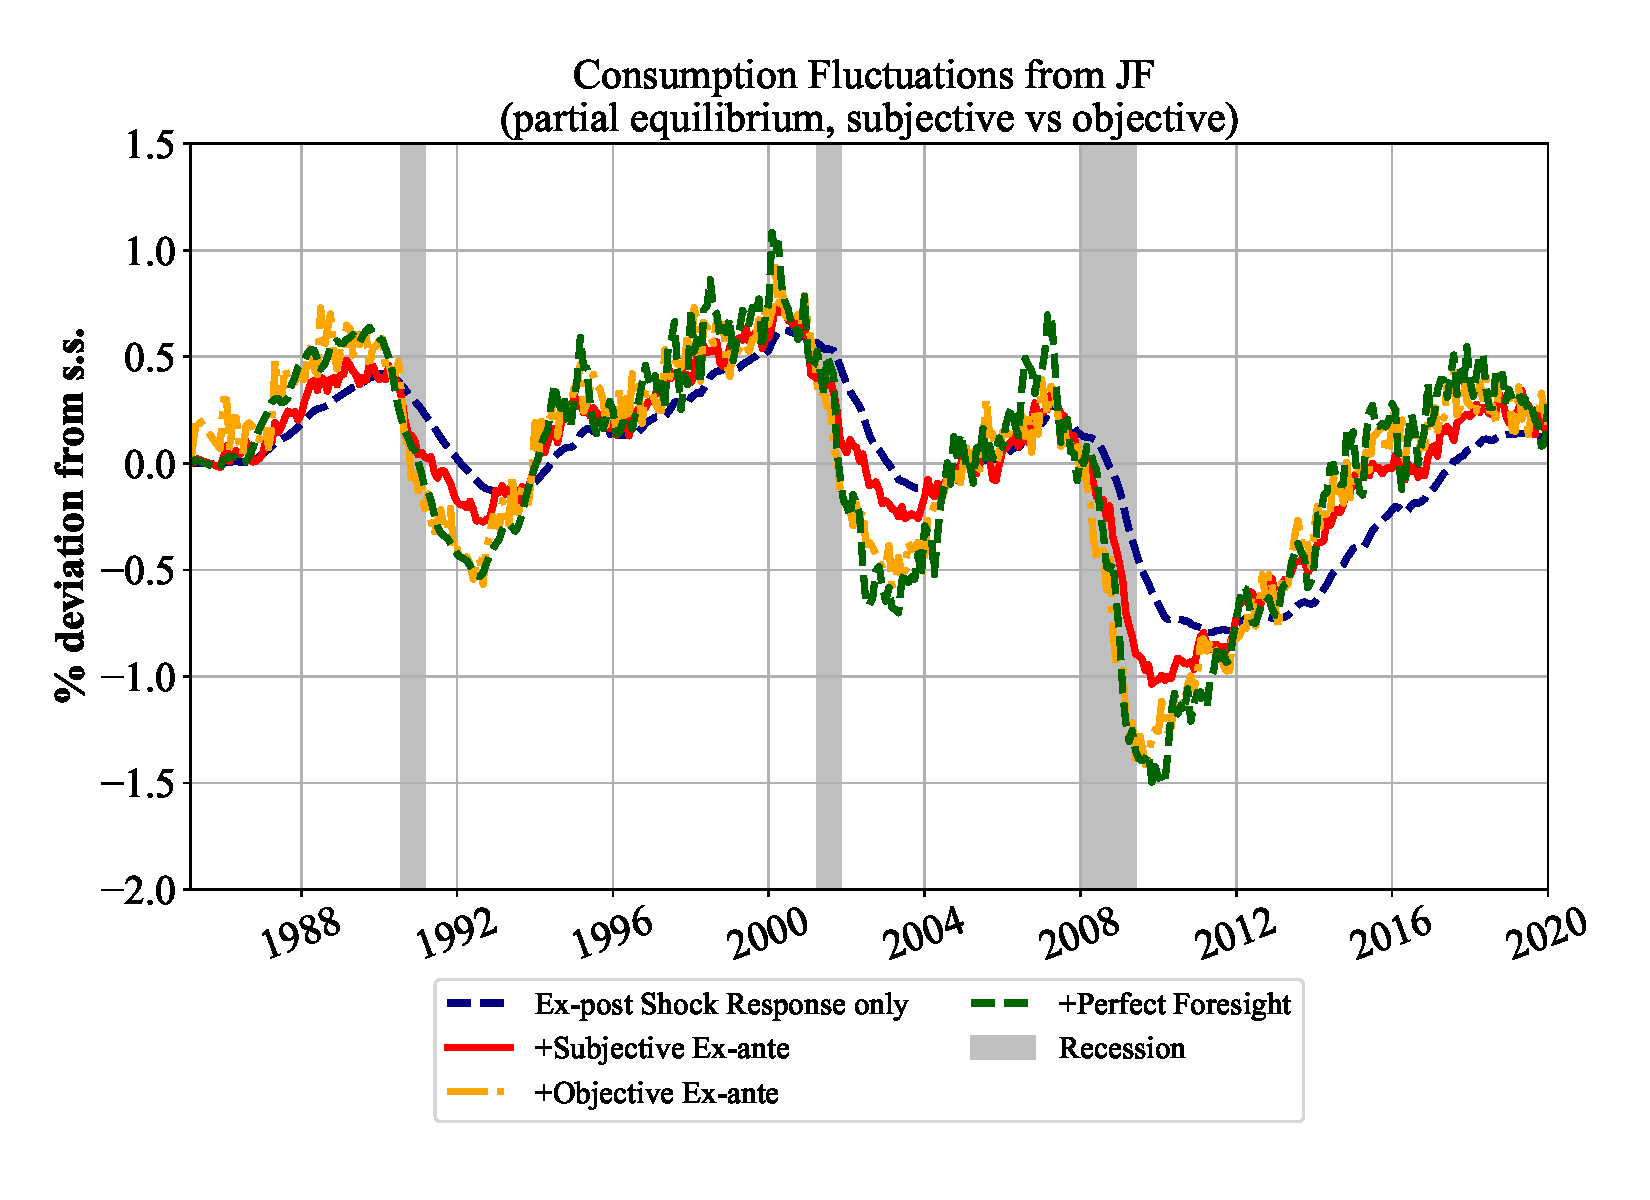
\includegraphics[width=\linewidth]{Figures/consumption_pe_JF_deviation_machine_as_rational_monthly.pdf}
   
    \end{subfigure}
    \hfill
    \begin{subfigure}{0.32\linewidth}
         \caption*{Combined}
        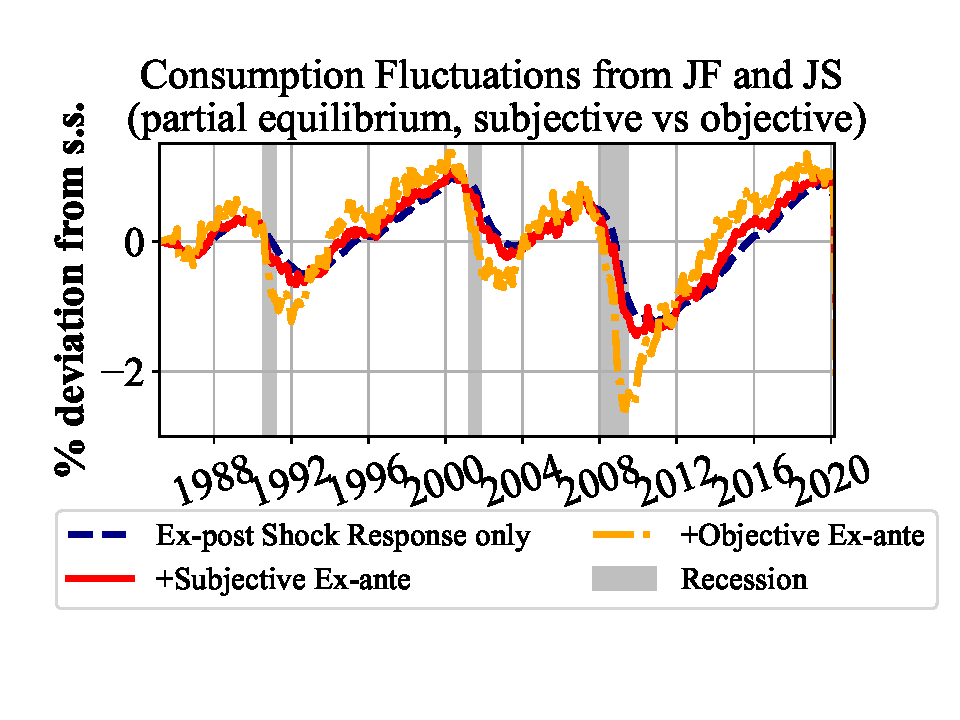
\includegraphics[width=\linewidth]{Figures/consumption_pe_JS_JF_deviation_machine_as_rational_monthly.pdf}
   
    \end{subfigure}

    \begin{flushleft}
        \footnotesize 
        Note: The figure compares the partial-equilibrium aggregate consumption deviations from its steady state simulated based on empirically estimated shocks to perceived job risk (subjective) and the real-time forecast risk (objective), in addition to the ex-post response to shocks to the realized job transition rates. The results are from a monthly variation of the baseline model set at the quarterly frequency.
    \end{flushleft}
\end{figure}

  \begin{figure}[ht]
    \centering
    \caption{\textbf{Monthly} Consumption Fluctuations due to Unemployment Risks: by Education}
    \label{fig:pe_decompose_sub_obj_educ_monthly}

    \begin{subfigure}{0.32\linewidth}
     \caption*{Low Education}
        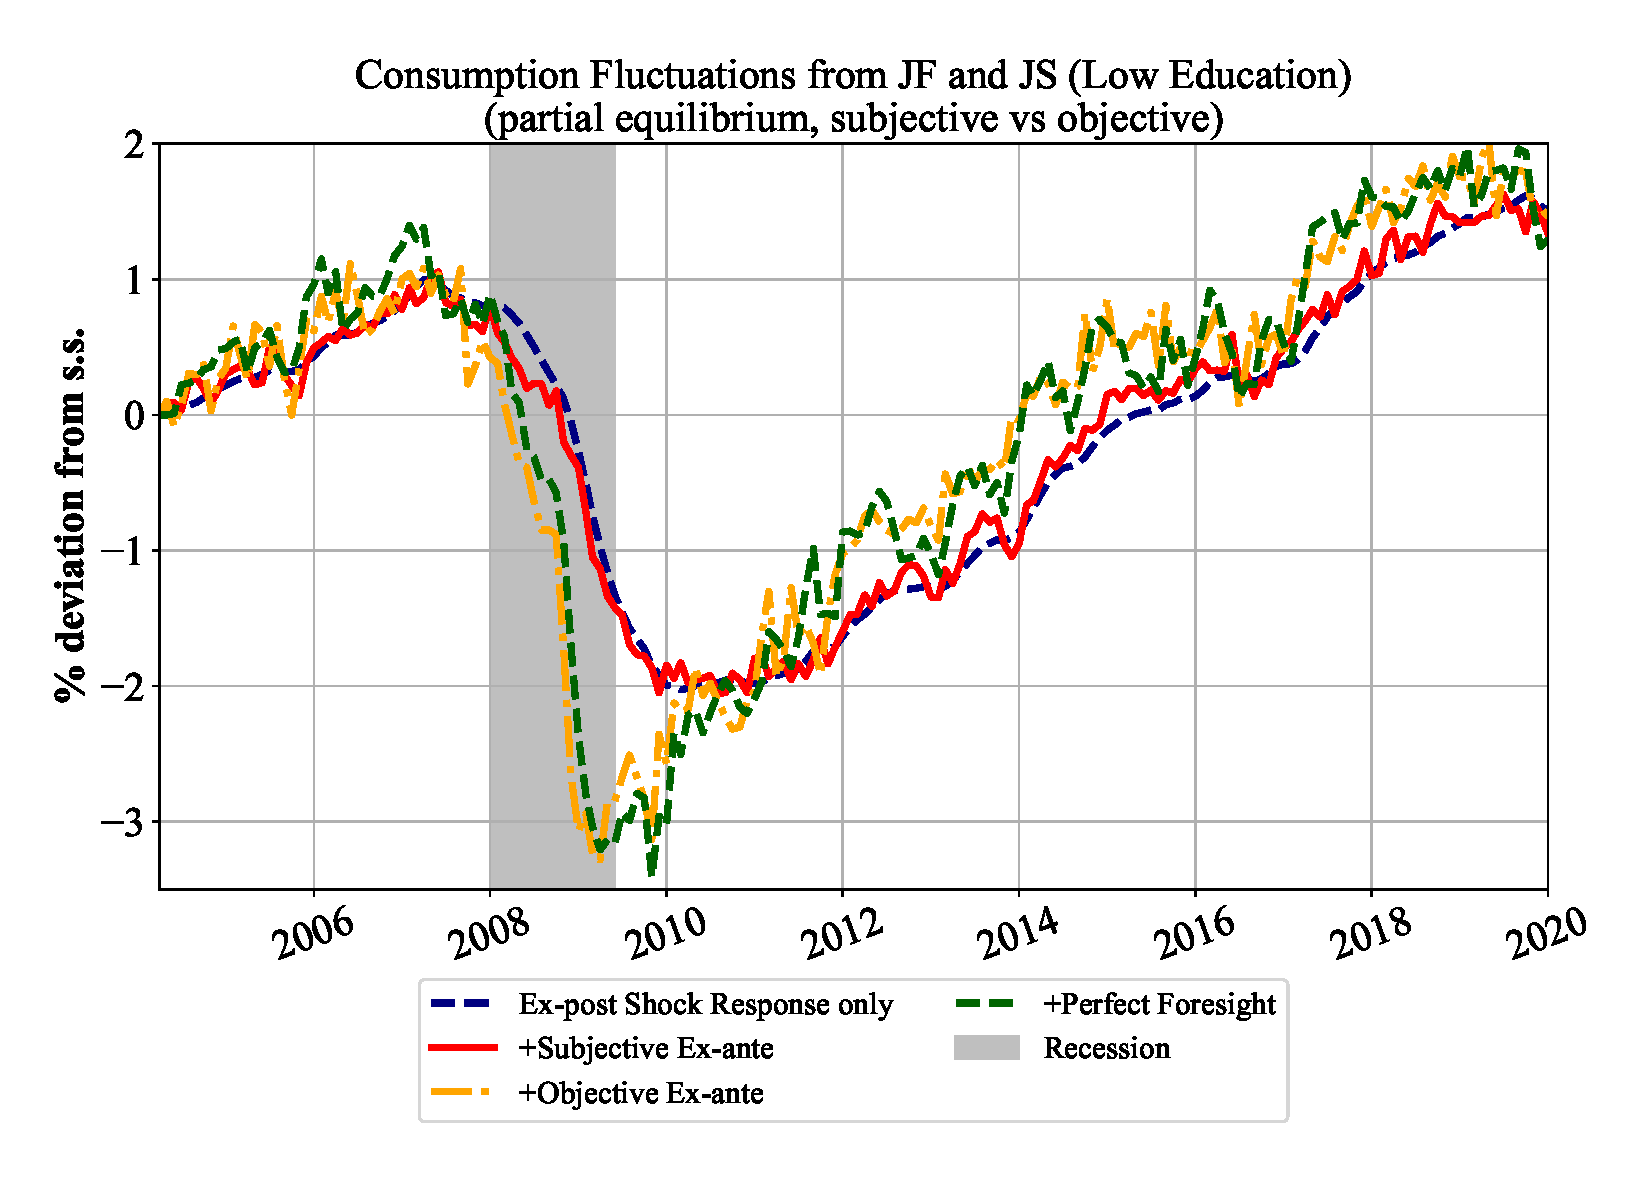
\includegraphics[width=\linewidth]{Figures/consumption_pe_JS_JF_deviation_machine_as_rational_LowEdu_monthly.pdf}
       
    \end{subfigure}
    \hfill
    \begin{subfigure}{0.32\linewidth}
     \caption*{Middle Education}
        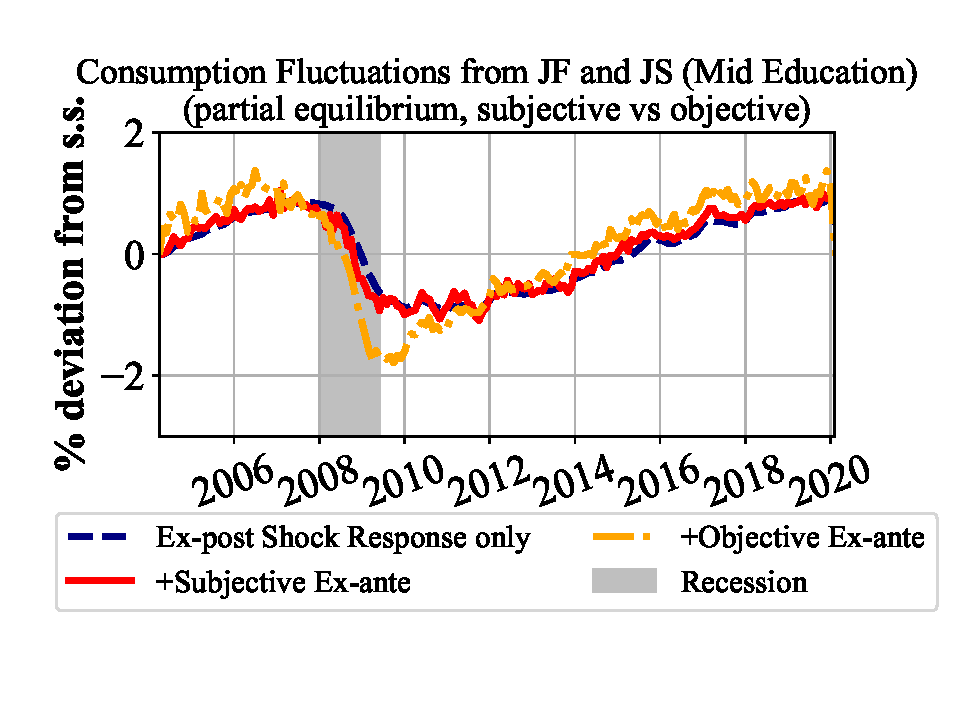
\includegraphics[width=\linewidth]{Figures/consumption_pe_JS_JF_deviation_machine_as_rational_MidEdu_monthly.pdf}
       
    \end{subfigure}
    \hfill
    \begin{subfigure}{0.32\linewidth}
      \caption*{High Education}
        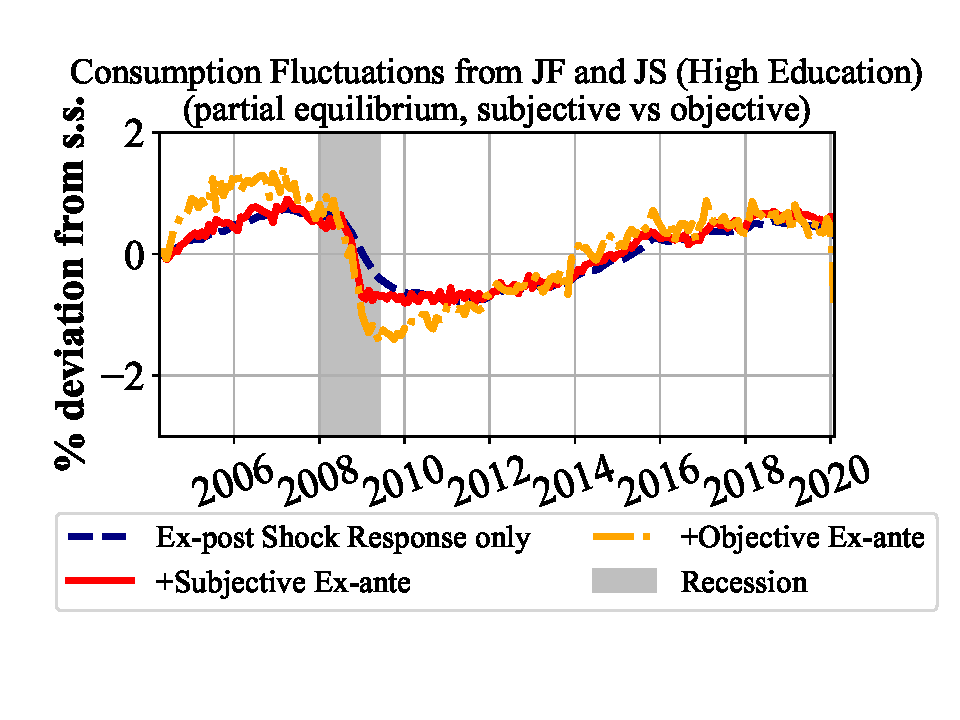
\includegraphics[width=\linewidth]{Figures/consumption_pe_JS_JF_deviation_machine_as_rational_HighEdu_monthly.pdf}
      
    \end{subfigure}

    \begin{flushleft}
        \footnotesize 
        Note: The figure compares for each education group their partial-equilibrium aggregate consumption deviations from its steady state simulated based on empirically estimated shocks to perceived job risk (subjective) and the real-time forecast risk (objective), in addition to the ex-post response to shocks to the realized job transition rates. The results are from the monthly version of the baseline model with modified assumptions.
    \end{flushleft}
\end{figure}